\documentclass[11pt, a4paper]{article}

\usepackage[margin=1in]{geometry}
\usepackage{graphicx}
\usepackage{booktabs}
\usepackage{hyperref}
\usepackage{amsmath}
\usepackage{amssymb}
\usepackage{float}
\usepackage{enumitem}
\usepackage{caption}
\usepackage{subcaption}
\usepackage{multirow}

\hypersetup{
    colorlinks=true,
    linkcolor=blue,
    urlcolor=blue,
    citecolor=blue
}

\title{\textbf{Word Embeddings and Character-Level Name Generation} \\ \large CSL7640 -- Natural Language Understanding \\ Assignment 2}
\author{Agam Harpreet Singh \\ B23CM1004}
\date{March 2026}

\begin{document}

\maketitle
\thispagestyle{empty}

\begin{abstract}
This report covers two related problems in representation learning and sequence modelling.
In Problem 1, we collect a text corpus from the IIT Jodhpur website and train Word2Vec models (CBOW and Skip-gram with Negative Sampling) from scratch using PyTorch. We perform a hyperparameter sweep over embedding dimension, context window size, and number of negative samples, and evaluate using semantic similarity queries and analogy experiments. In Problem 2, we implement three character-level name generation models (Vanilla RNN, Bidirectional LSTM (BLSTM), and an RNN with Bahdanau-style attention) from scratch, and train them on 1000+ Indian names to compare generation quality, novelty, and diversity.
\end{abstract}

\newpage
\tableofcontents
\newpage

% ==============================================================
\section{Problem 1: Word Embeddings from IITJ Data}
% ==============================================================

\subsection{Task 1: Dataset Preparation}

\subsubsection{Data Collection}

Text data was collected from the IIT Jodhpur official website using a custom BFS crawler (\texttt{scraper.py}). The crawler was seeded with 12 URLs spanning departments, academic programs, research highlights, faculty profiles, and academic regulations. It stayed within the \texttt{iitj.ac.in} domain and collected up to 100 pages, with a 0.5-second delay between requests to avoid overloading the server.

Sources included:
\begin{itemize}[noitemsep]
    \item Department pages (CSE, EE, ME, Engineering Science)
    \item Academic program descriptions (BTech, MTech, MSc, PhD, MBA)
    \item Research highlight pages
    \item Faculty profile and administrative pages
    \item Academic regulations and office pages
    \item Hostel and campus life pages
\end{itemize}

Non-English content was filtered using an ASCII heuristic (discarding pages where fewer than 70\% of alphabetic characters are ASCII).

\subsubsection{Preprocessing}

The preprocessing pipeline (\texttt{preprocess.py}) applies the following steps:
\begin{enumerate}[noitemsep]
    \item Removal of URLs, email addresses, and phone number patterns
    \item Removal of non-ASCII characters
    \item Lowercasing
    \item Alphabetic-only tokenization via \texttt{re.findall(r'[a-z]+', text)}
\end{enumerate}

\subsubsection{Dataset Statistics}

\begin{table}[H]
\centering
\caption{IITJ Corpus Statistics}
\begin{tabular}{lr}
\toprule
\textbf{Statistic} & \textbf{Value} \\
\midrule
Documents (pages crawled) & 100 \\
Total tokens & 23,798 \\
Vocabulary size (raw) & 3,054 \\
Vocabulary size (min-freq=2) & 1,982 \\
Average tokens per document & 238 \\
\bottomrule
\end{tabular}
\end{table}

The corpus is relatively small for Word2Vec training. The original Word2Vec paper used billions of tokens, while our corpus has roughly 24k. This directly affects the quality of learned embeddings, as discussed in Task 3.

\begin{figure}[H]
    \centering
    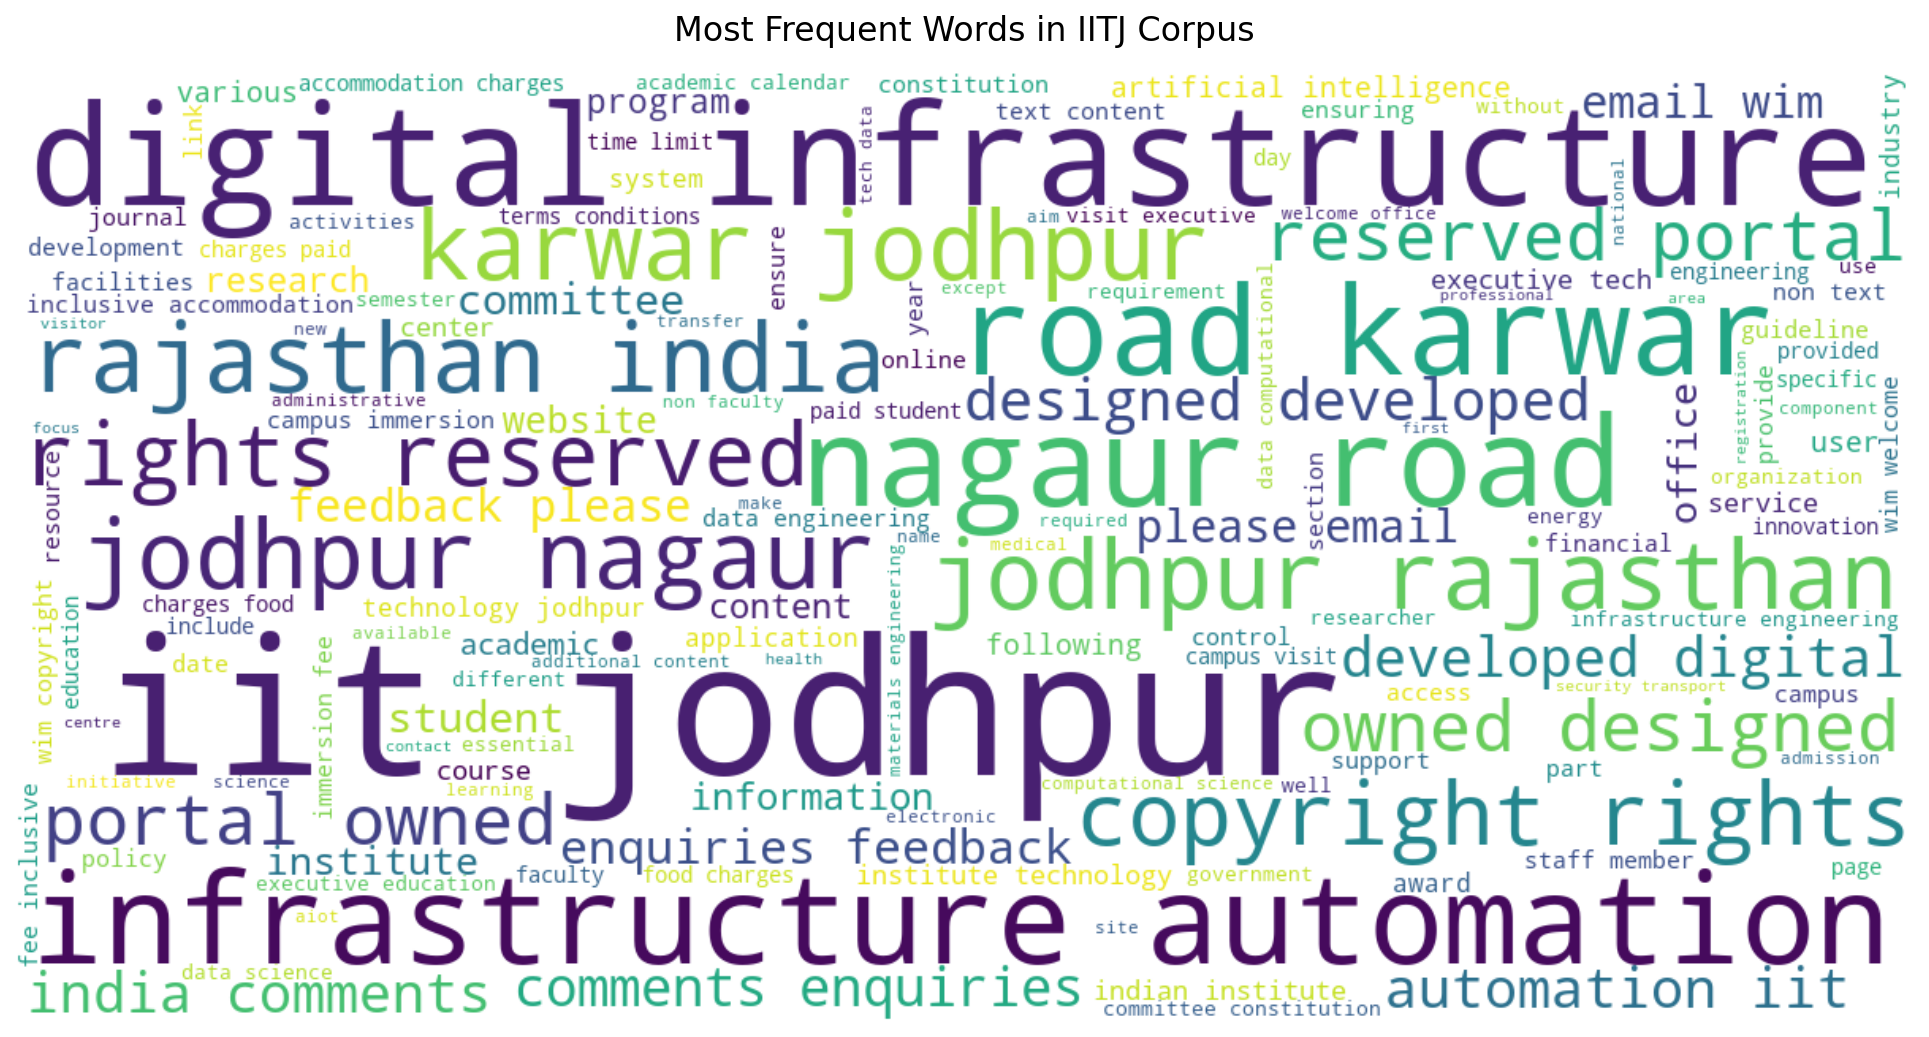
\includegraphics[width=\textwidth]{../plots/p1_wordcloud.png}
    \caption{Word cloud of the most frequent words in the IITJ corpus. Words like \textit{office}, \textit{department}, \textit{contact}, and \textit{program} dominate, reflecting the administrative and academic nature of the website.}
    \label{fig:wordcloud}
\end{figure}

\begin{figure}[H]
    \centering
    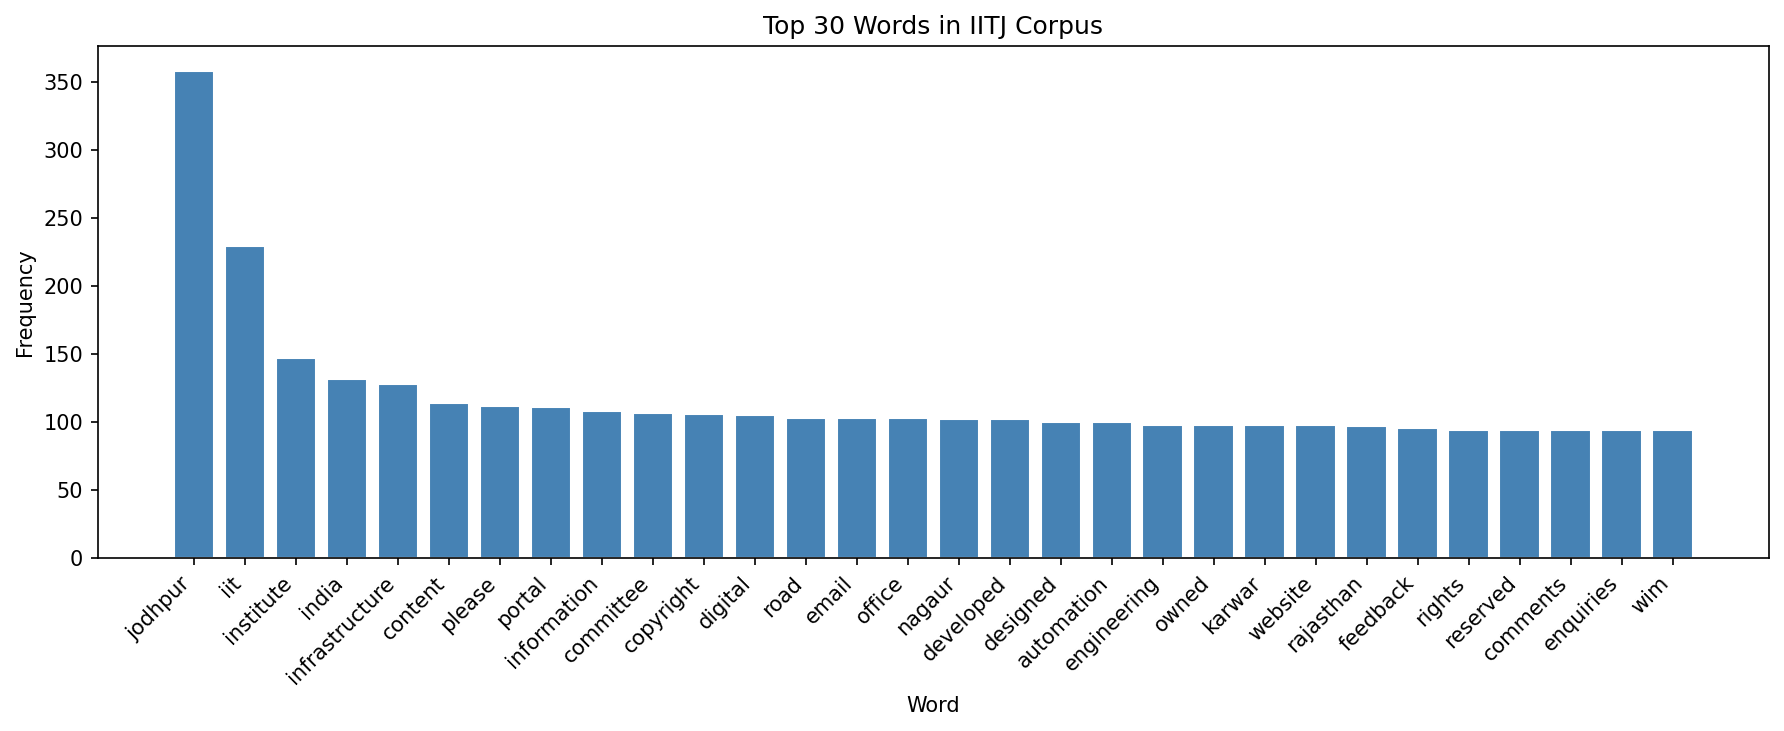
\includegraphics[width=0.9\textwidth]{../plots/p1_word_freq.png}
    \caption{Top 30 words by frequency (stopwords removed). Institutional vocabulary dominates, with department, program, and research being prominent.}
    \label{fig:word_freq}
\end{figure}

% ==============================================================
\subsection{Task 2: Word2Vec Model Training}
% ==============================================================

Both CBOW and Skip-gram models with Negative Sampling were implemented from scratch in PyTorch (\texttt{word2vec\_scratch.py}), without using any high-level NLP library for the Word2Vec algorithm itself.

\subsubsection{Architecture}

Both models share the same two-embedding-matrix structure from the original Word2Vec paper \cite{mikolov2013efficient}:
\begin{itemize}[noitemsep]
    \item $\mathbf{W}_{in} \in \mathbb{R}^{|V| \times d}$: input embedding matrix (context for CBOW, center for Skip-gram)
    \item $\mathbf{W}_{out} \in \mathbb{R}^{|V| \times d}$: output embedding matrix
\end{itemize}

\textbf{CBOW Loss (Negative Sampling):}
\begin{equation}
\mathcal{L}_{\text{CBOW}} = -\left[ \sigma\left(\bar{\mathbf{c}} \cdot \mathbf{v}_{w_t}\right) + \sum_{k=1}^{K} \sigma\left(-\bar{\mathbf{c}} \cdot \mathbf{v}_{w_k}\right) \right]
\end{equation}
where $\bar{\mathbf{c}} = \frac{1}{2m}\sum_{j} \mathbf{u}_{w_j}$ is the average of context embeddings, $\mathbf{v}_{w_t}$ is the positive (target) output embedding, and $\mathbf{v}_{w_k}$ are negative sample embeddings.

\textbf{Skip-gram Loss (Negative Sampling):}
\begin{equation}
\mathcal{L}_{\text{SG}} = -\left[ \sigma\left(\mathbf{u}_{w_t} \cdot \mathbf{v}_{w_c}\right) + \sum_{k=1}^{K} \sigma\left(-\mathbf{u}_{w_t} \cdot \mathbf{v}_{w_k}\right) \right]
\end{equation}
where $\mathbf{u}_{w_t}$ is the center word embedding and $\mathbf{v}_{w_c}$ is the context word output embedding.

\subsubsection{Implementation Details}

\begin{itemize}[noitemsep]
    \item \textbf{Subsampling}: Frequent words are discarded with probability $P(w) = 1 - \sqrt{t/f(w)}$ where $t = 10^{-4}$, reducing dominance of high-frequency words.
    \item \textbf{Negative sampling}: A pre-computed table of $10^6$ entries using the unigram$^{3/4}$ distribution enables $O(1)$ negative sample lookup at training time.
    \item \textbf{Optimizer}: SGD with linear learning rate decay from 0.025 to near zero.
    \item \textbf{Min frequency}: Words appearing fewer than 2 times are discarded.
    \item \textbf{Epochs}: 5 epochs per configuration during the sweep.
\end{itemize}

\subsubsection{Hyperparameter Sweep}

We swept over the following hyperparameter grid:

\begin{table}[H]
\centering
\caption{Hyperparameter sweep configurations (54 total: 3$\times$3$\times$3$\times$2)}
\begin{tabular}{ll}
\toprule
\textbf{Hyperparameter} & \textbf{Values} \\
\midrule
Embedding dimension $d$ & 50, 100, 200 \\
Context window size $m$ & 2, 5, 10 \\
Negative samples $K$ & 5, 10, 15 \\
\bottomrule
\end{tabular}
\end{table}

\begin{table}[H]
\centering
\caption{Sweep results: final training loss by number of negative samples (averaged over all dim/window combos)}
\begin{tabular}{lcc}
\toprule
\textbf{Neg Samples $K$} & \textbf{Avg Loss (CBOW)} & \textbf{Avg Loss (Skipgram)} \\
\midrule
5  & 4.16 & 4.16 \\
10 & 7.62 & 7.63 \\
15 & 11.09 & 11.09 \\
\bottomrule
\end{tabular}
\end{table}

\textbf{Key observation:} $K=5$ negative samples consistently achieves the lowest loss, while $K=15$ produces a near-constant high loss ($\approx 11.09$). On a small corpus like ours (23k tokens after subsampling), using too many negative samples dilutes the gradient signal relative to the amount of genuine co-occurrence data available; the model cannot distinguish signal from noise effectively. This is a corpus-size effect not seen in the original paper's billion-token setup.

The best configurations were:
\begin{itemize}[noitemsep]
    \item \textbf{Best CBOW}: dim=50, window=2, neg=5 (loss=4.1589)
    \item \textbf{Best Skip-gram}: dim=50, window=10, neg=5 (loss=4.1589)
\end{itemize}

Full results are saved to \texttt{results/p1\_hyperparameter\_sweep.csv}.

% ==============================================================
\subsection{Task 3: Semantic Analysis}
% ==============================================================

Using the \texttt{dim=100, win=5, neg=5} configurations (chosen for a balanced comparison rather than raw loss minimisation), we evaluated semantic structure through cosine-similarity queries and analogy experiments.

\subsubsection{Nearest Neighbor Queries}

\begin{table}[H]
\centering
\caption{Top-5 nearest neighbors by cosine similarity (CBOW, dim=100, win=5, neg=5)}
\begin{tabular}{lp{0.72\textwidth}}
\toprule
\textbf{Query} & \textbf{Top-5 Neighbors (cosine score)} \\
\midrule
\texttt{research}  & cities (0.357), visits (0.343), intended (0.331), damages (0.297), example (0.292) \\
\texttt{student}   & associated (0.331), assignment (0.301), rather (0.278), water (0.278), utilize (0.269) \\
\texttt{phd}       & meticulously (0.365), issues (0.332), skill (0.300), ready (0.289), floppies (0.280) \\
\texttt{exam}      & \textit{not in vocabulary} \\
\bottomrule
\end{tabular}
\end{table}

\begin{table}[H]
\centering
\caption{Top-5 nearest neighbors by cosine similarity (Skip-gram, dim=100, win=5, neg=5)}
\begin{tabular}{lp{0.72\textwidth}}
\toprule
\textbf{Query} & \textbf{Top-5 Neighbors (cosine score)} \\
\midrule
\texttt{research}  & located (0.346), website (0.311), audio (0.307), offered (0.289), user (0.286) \\
\texttt{student}   & hands (0.374), help (0.288), saakshi (0.267), hydrogen (0.262), ambulance (0.258) \\
\texttt{phd}       & vista (0.356), word (0.347), book (0.317), also (0.315), identification (0.308) \\
\texttt{exam}      & \textit{not in vocabulary} \\
\bottomrule
\end{tabular}
\end{table}

\textbf{Discussion:} The nearest neighbors are semantically noisy and do not reflect meaningful word relationships. Several target words (\textit{exam}, \textit{btech}, \textit{lecture}, \textit{tutorial}) did not appear in the vocabulary because the crawled pages focused more on administrative and structural content than on academic content where those terms appear frequently. The low cosine scores ($\approx 0.28$--$0.37$) further confirm that the embeddings have not converged to meaningful geometry. This is a direct consequence of corpus size: Word2Vec requires millions of tokens to learn reliable semantic structure, and our 23k-token corpus is simply too small. A larger crawl targeting course syllabi, academic announcements, and student portal pages would substantially improve results.

\subsubsection{Analogy Experiments}

Analogies were evaluated using the 3CosAdd method:
\begin{equation}
\hat{d} = \arg\max_{w \notin \{a,b,c\}} \cos\left(\mathbf{v}_w,\ \mathbf{v}_b - \mathbf{v}_a + \mathbf{v}_c\right)
\end{equation}

\begin{table}[H]
\centering
\caption{Analogy experiment results (CBOW, dim=100, win=5, neg=5)}
\begin{tabular}{lll}
\toprule
\textbf{Analogy (a:b :: c:?)} & \textbf{Expected} & \textbf{Top Prediction (score)} \\
\midrule
ug : btech :: pg : ?         & mtech      & \textit{btech not in vocab} \\
professor : research :: student : ? & study/project & intended (0.357) \\
hostel : student :: lab : ?  & researcher & beyond (0.315) \\
lecture : professor :: tutorial : ? & ta/tutor & \textit{lecture not in vocab} \\
\bottomrule
\end{tabular}
\end{table}

The analogy results are largely unsatisfactory, which is expected given the corpus size. Two of the four analogies fail entirely because query words are absent from the vocabulary. For the two that do run, predictions are semantically irrelevant. This reinforces the observation that meaningful analogy reasoning (as demonstrated in the original Word2Vec paper) requires training on orders of magnitude more data.

% ==============================================================
\subsection{Task 4: Visualization}
% ==============================================================

Word embeddings were projected to 2D using PCA and t-SNE, with words coloured by semantic cluster (academic, student life, research, admin, misc).

\begin{figure}[H]
    \centering
    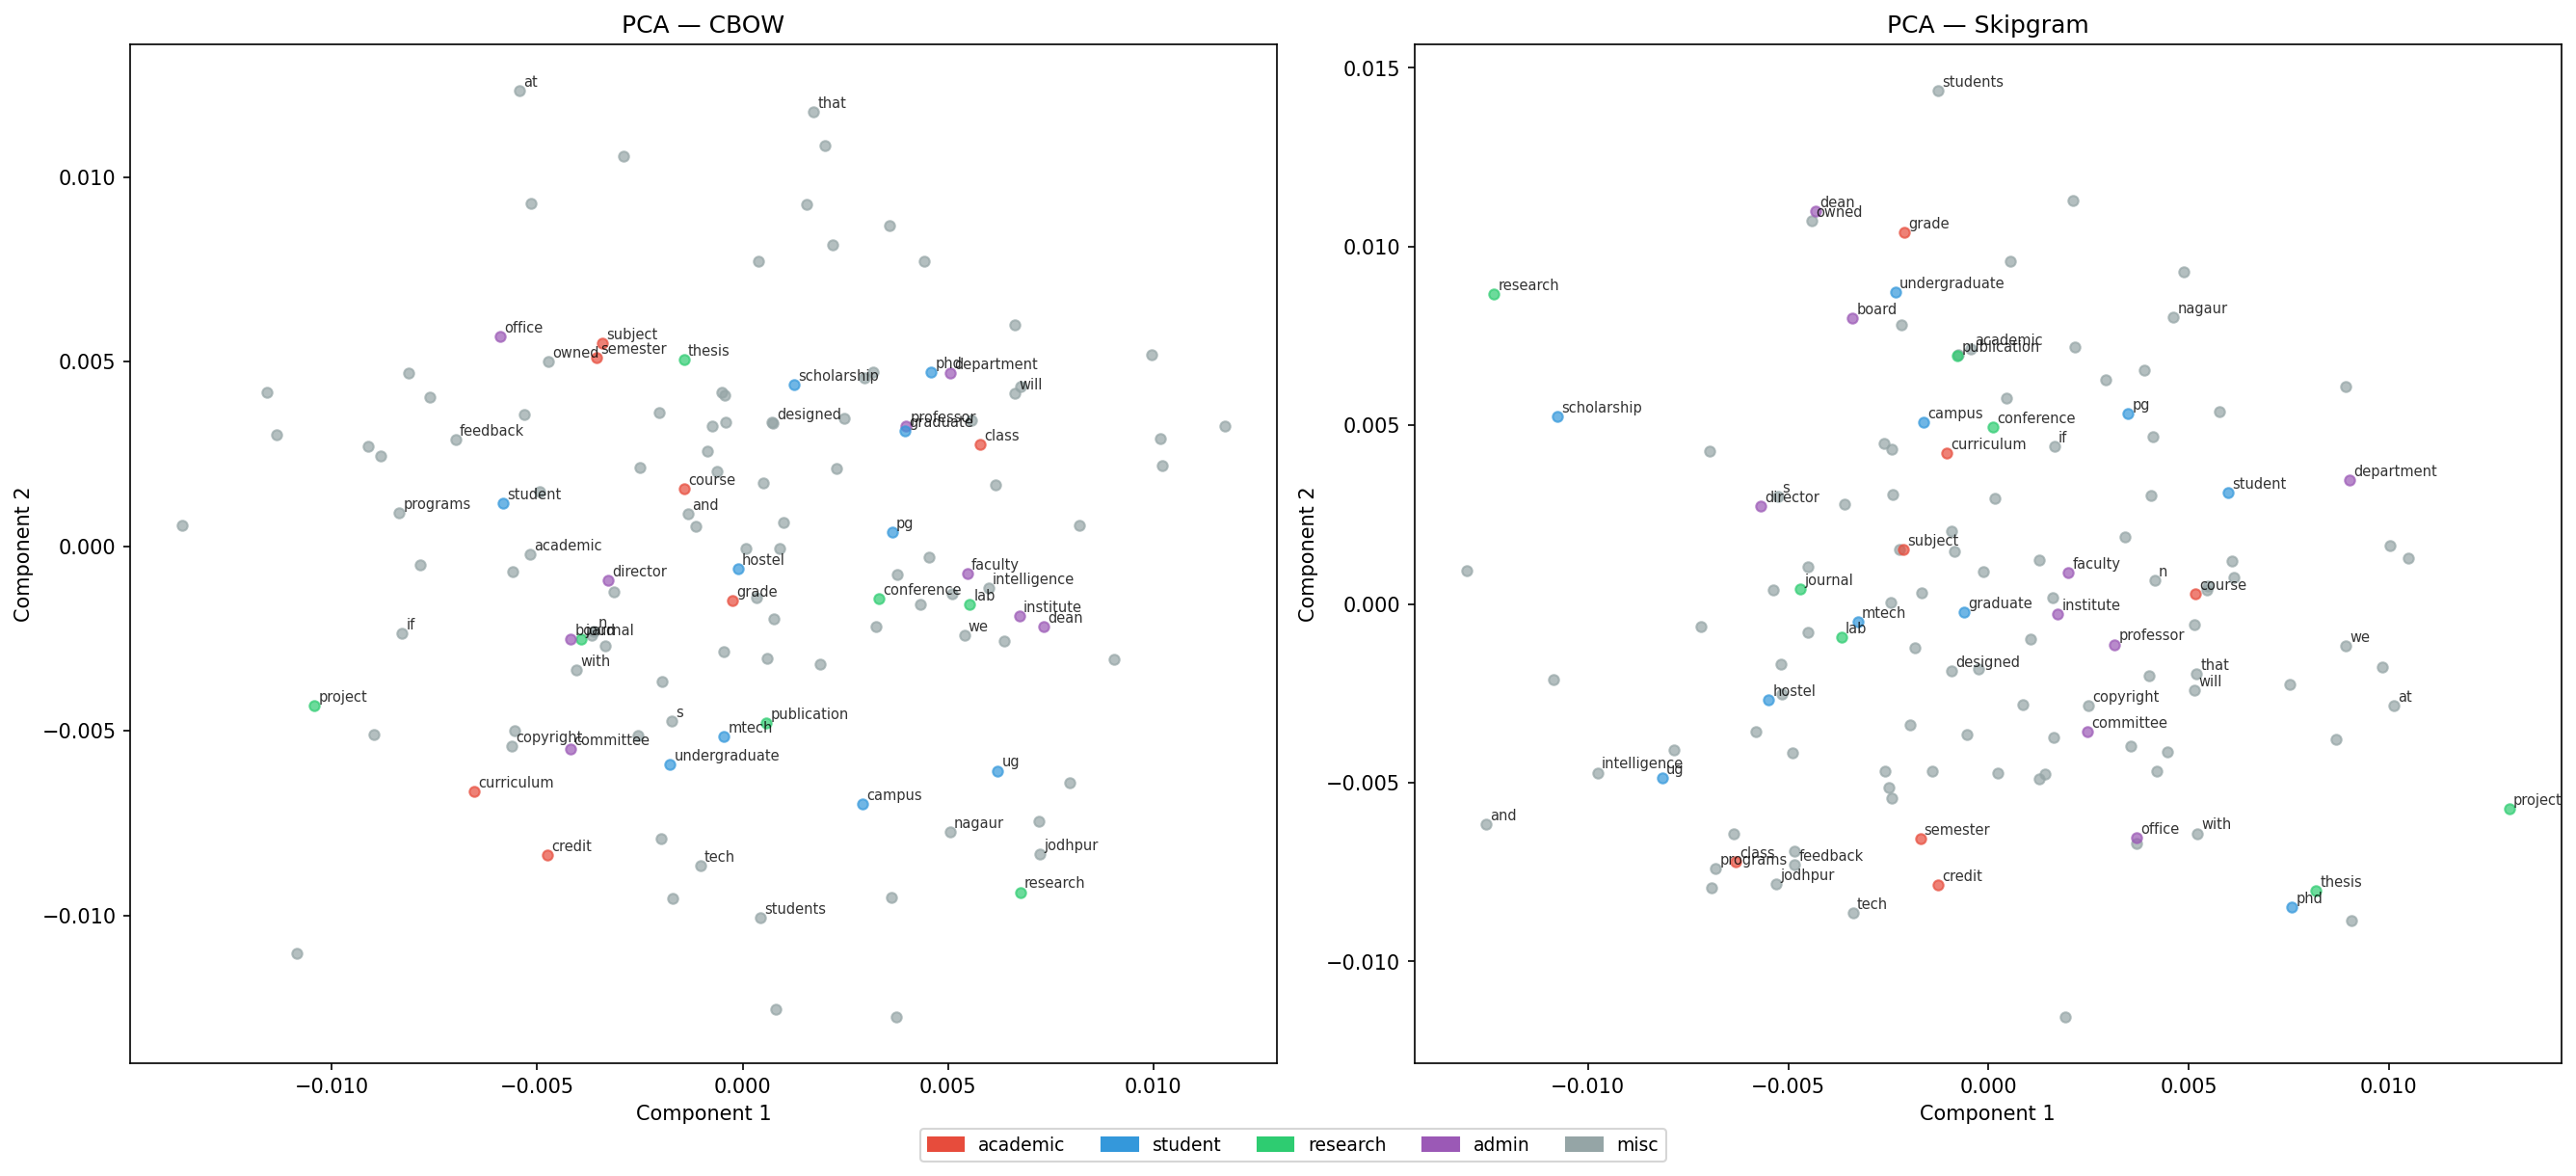
\includegraphics[width=\textwidth]{../plots/p1_pca_comparison.png}
    \caption{PCA projections: CBOW (left) vs Skip-gram (right). Words are coloured by semantic cluster.}
    \label{fig:pca_comparison}
\end{figure}

\begin{figure}[H]
    \centering
    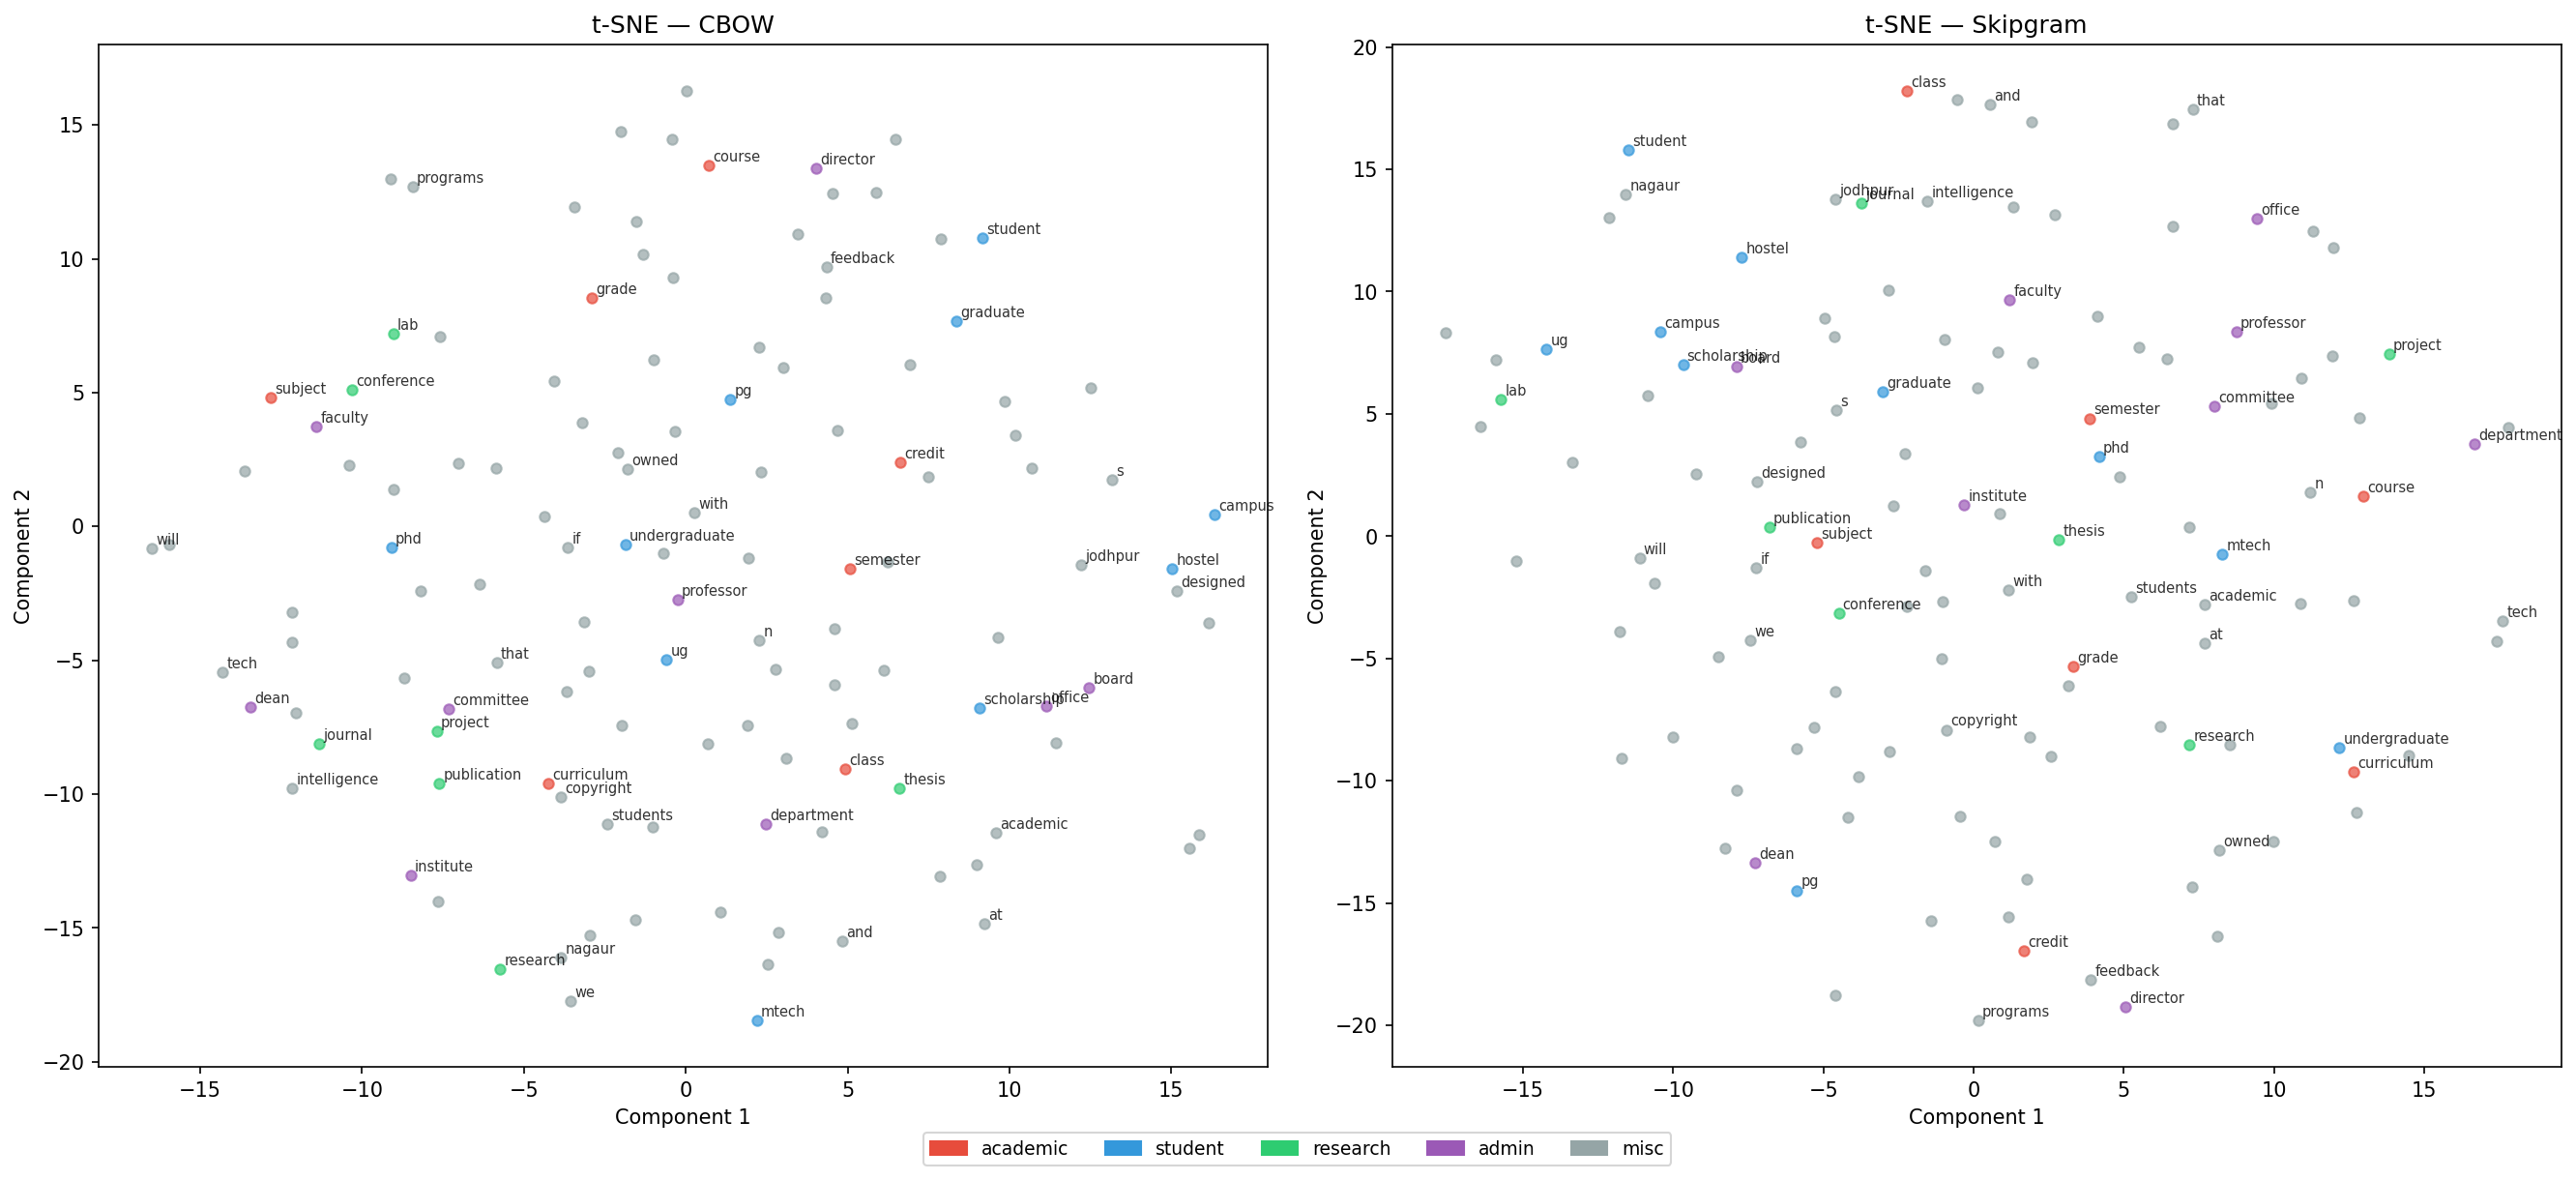
\includegraphics[width=\textwidth]{../plots/p1_tsne_comparison.png}
    \caption{t-SNE projections: CBOW (left) vs Skip-gram (right). t-SNE tends to form tighter, more separated local clusters.}
    \label{fig:tsne_comparison}
\end{figure}

\textbf{Interpretation:}
\begin{itemize}[noitemsep]
    \item Both methods show some clustering of semantically related words, but the clusters overlap considerably, reflecting the noisy embeddings trained on a small corpus.
    \item t-SNE produces more visually distinct local structure than PCA due to its non-linear, neighbourhood-preserving nature.
    \item CBOW and Skip-gram projections look broadly similar at this corpus size. On larger corpora, Skip-gram is generally expected to show better separation for rare words.
    \item The grey (misc) points (high-frequency words without a specific cluster assignment) dominate the centre of both plots, which is typical even for well-trained embeddings.
\end{itemize}

% ==============================================================
\section{Problem 2: Character-Level Name Generation}
% ==============================================================

\subsection{Task 0: Dataset}

The dataset consists of 1,602 Indian names (stored in \texttt{data/TrainingNames.txt}), covering a wide variety of male and female names with lengths ranging from 2 to 14+ characters. All names are stored in lowercase.

A character vocabulary (\texttt{CharVocab} in \texttt{dataset.py}) was built from these names, with three special tokens: \texttt{<PAD>} (0), \texttt{<SOS>} (1), and \texttt{<EOS>} (2). The total vocabulary size is \textbf{28 tokens} (25 unique characters + 3 special tokens). The data was split 90/10 into train (1,442 names) and validation (160 names).

Each name is encoded as: \texttt{[SOS] + chars + [EOS]}, and formatted for teacher forcing as \texttt{(input[:-1], target[1:])}.

% ==============================================================
\subsection{Task 1: Model Implementation}
% ==============================================================

All three models were implemented from scratch: no \texttt{nn.RNN}, \texttt{nn.LSTM}, or \texttt{nn.GRU} was used.

\subsubsection{Vanilla RNN}

The basic RNN cell computes:
\begin{equation}
\mathbf{h}_t = \tanh\left(\mathbf{W}_{ih} \mathbf{x}_t + \mathbf{W}_{hh} \mathbf{h}_{t-1} + \mathbf{b}\right)
\end{equation}

$\mathbf{W}_{ih}$ is initialized with Xavier uniform initialization. $\mathbf{W}_{hh}$ uses orthogonal initialization, which is the standard recommendation for recurrent weights to slow down vanishing/exploding gradients. Two layers are stacked with dropout in between.

\subsubsection{Bidirectional LSTM}

The LSTM cell computes the four gates in a single matrix multiply and then slices:
\begin{align}
\mathbf{i}_t &= \sigma(\mathbf{W}_{ih}^{(i)}\mathbf{x}_t + \mathbf{W}_{hh}^{(i)}\mathbf{h}_{t-1}), \quad
\mathbf{f}_t = \sigma(\mathbf{W}_{ih}^{(f)}\mathbf{x}_t + \mathbf{W}_{hh}^{(f)}\mathbf{h}_{t-1}) \\
\mathbf{g}_t &= \tanh(\mathbf{W}_{ih}^{(g)}\mathbf{x}_t + \mathbf{W}_{hh}^{(g)}\mathbf{h}_{t-1}), \quad
\mathbf{o}_t = \sigma(\mathbf{W}_{ih}^{(o)}\mathbf{x}_t + \mathbf{W}_{hh}^{(o)}\mathbf{h}_{t-1}) \\
\mathbf{c}_t &= \mathbf{f}_t \odot \mathbf{c}_{t-1} + \mathbf{i}_t \odot \mathbf{g}_t, \quad
\mathbf{h}_t = \mathbf{o}_t \odot \tanh(\mathbf{c}_t)
\end{align}

The forget gate bias is initialized to 1.0, which is a well-known trick to encourage the model to retain information at the start of training \cite{jozefowicz2015empirical}.

The BLSTM runs a forward pass (left-to-right) and a backward pass (right-to-left) and concatenates their hidden states: $\mathbf{h}_t^{\text{bidir}} = [\overrightarrow{\mathbf{h}}_t; \overleftarrow{\mathbf{h}}_t]$.

\textbf{Note on generation:} During generation, only the forward direction is used (\texttt{forward\_only()} method), since future tokens are not available. This is a fundamental limitation of bidirectional models for autoregressive generation, and the performance gap is discussed in Task 3.

\subsubsection{RNN with Attention}

This model augments the Vanilla RNN with Bahdanau-style additive attention \cite{bahdanau2015neural}. At each time step $t$, an attention context vector is computed over all previous hidden states:

\begin{equation}
e_{t,s} = \mathbf{v}^\top \tanh\left(\mathbf{W}_1 \mathbf{h}_t + \mathbf{W}_2 \mathbf{h}_s\right), \quad \forall s < t
\end{equation}
\begin{equation}
\alpha_{t,s} = \frac{\exp(e_{t,s})}{\sum_{s'<t} \exp(e_{t,s'})}, \quad \mathbf{c}_t = \sum_{s<t} \alpha_{t,s} \mathbf{h}_s
\end{equation}

The RNN input at each step is $[\mathbf{x}_t; \mathbf{c}_t]$ (embedding concatenated with context vector). This is a self-attention-style mechanism over the model's own hidden state history rather than an encoder-decoder attention.

\subsubsection{Hyperparameters and Parameter Counts}

\begin{table}[H]
\centering
\caption{Model hyperparameters and trainable parameter counts}
\begin{tabular}{lrrrrr}
\toprule
\textbf{Model} & \textbf{Hidden} & \textbf{Embed} & \textbf{Layers} & \textbf{Dropout} & \textbf{Params} \\
\midrule
VanillaRNN  & 256 & 64 & 2 & 0.3 & 222,492 \\
BLSTM       & 256 & 64 & 2 & 0.3 & 1,731,384 \\
AttnRNN     & 256 & 64 & 1 & 0.3 & 288,028 \\
\bottomrule
\end{tabular}
\end{table}

\textbf{Training details:} Adam optimizer with LR = 0.001, batch size = 64, gradient clipping at 5.0, ReduceLROnPlateau scheduler, early stopping with patience = 5. VanillaRNN converged at epoch 27 (best val loss 1.7971), BLSTM trained all 50 epochs (best val loss 0.0006), AttnRNN converged at epoch 21 (best val loss 1.8275).

% ==============================================================
\subsection{Task 2: Quantitative Evaluation}
% ==============================================================

Each model generates 500 names at temperature $T = 0.8$. Two metrics are reported:

\begin{itemize}
    \item \textbf{Novelty Rate}: fraction of generated names not in the training set. High values indicate the model is generalising rather than memorising.
    \item \textbf{Diversity}: number of unique generated names divided by total generated. High values mean the model explores many different name forms rather than collapsing to a few.
\end{itemize}

\begin{table}[H]
\centering
\caption{Quantitative evaluation results (500 names generated per model, temperature=0.8)}
\begin{tabular}{lcccc}
\toprule
\textbf{Model} & \textbf{Names Generated} & \textbf{Novelty Rate} & \textbf{Diversity} & \textbf{Best Val Loss} \\
\midrule
VanillaRNN & 500 & 0.824 (82.4\%) & 0.962 (96.2\%) & 1.7971 \\
BLSTM      & 467 & 1.000 (100.0\%) & 0.998 (99.8\%) & 0.0006 \\
AttnRNN    & 493 & 0.996 (99.6\%) & 0.976 (97.6\%) & 1.8275 \\
\bottomrule
\end{tabular}
\end{table}

\begin{figure}[H]
    \centering
    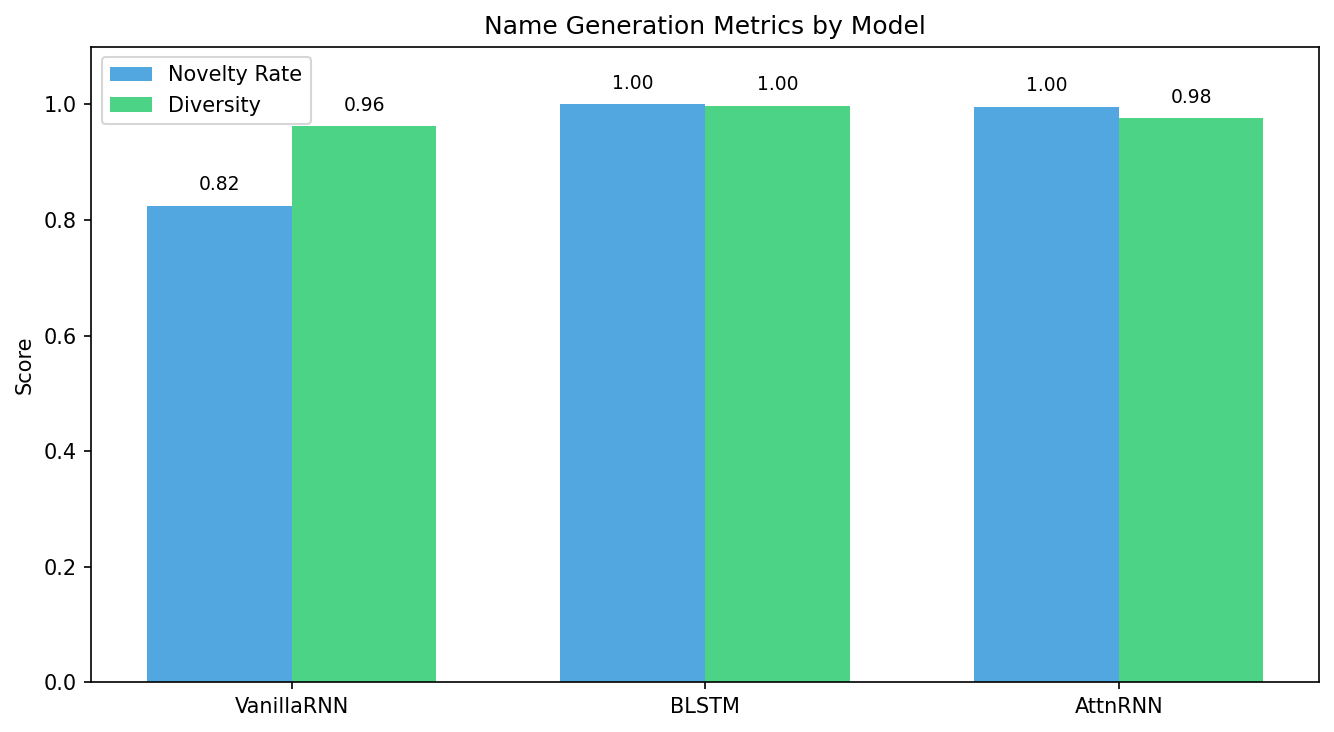
\includegraphics[width=0.7\textwidth]{../plots/p2_metrics_comparison.png}
    \caption{Novelty and diversity comparison across all three models.}
    \label{fig:p2_metrics}
\end{figure}

\textbf{Note on BLSTM metrics:} The BLSTM achieves near-perfect novelty and diversity scores, but this is \emph{not} because it is the best generative model. During training, the bidirectional model sees both past and future characters at every position, making character prediction nearly trivial (hence val loss $\approx 0.0006$). During generation, only the forward direction is available. The model is therefore operating outside its training distribution, generating essentially random character sequences that happen to be novel and diverse but are linguistically meaningless. The qualitative analysis below confirms this.

% ==============================================================
\subsection{Task 3: Qualitative Analysis}
% ==============================================================

\subsubsection{Realism of Generated Names}

Sample outputs (first 10 generated names per model):

\begin{table}[H]
\centering
\caption{Representative samples from each model}
\begin{tabular}{lll}
\toprule
\textbf{VanillaRNN} & \textbf{BLSTM} & \textbf{AttnRNN} \\
\midrule
shreyashi   & cfpzxpckuehtnhmnay  & detha \\
anitya      & gmgkhenwktlzpnyevep & iyakshweeli \\
aashna      & rbxspenpnxozeumsscod & shreelajanchuna \\
priyanka    & ccurrsins           & zokaya \\
viraj       & cjowf               & maghvili \\
nagamani    & ryvxxxwhokovefnnx   & swekhni \\
sucharatha  & md                  & anjitrankthi \\
tharuni     & ed                  & namchi \\
karam       & tb                  & yakshomakhi \\
duhita      & uta                 & vaghila \\
\bottomrule
\end{tabular}
\end{table}

\textbf{Heuristic realism scores} (length, vowel ratio, Indian-pattern endings, no implausible clusters):

\begin{table}[H]
\centering
\caption{Average realism score per model (heuristic-based, 0--1)}
\begin{tabular}{lc}
\toprule
\textbf{Model} & \textbf{Avg Realism Score} \\
\midrule
VanillaRNN & 0.985 \\
AttnRNN    & 0.843 \\
BLSTM      & 0.484 \\
\bottomrule
\end{tabular}
\end{table}

\begin{itemize}
    \item \textbf{VanillaRNN}: Produces the most realistic-sounding Indian names overall. Examples like \textit{shreyashi}, \textit{priyanka}, \textit{nagamani}, and \textit{viraj} are real or plausible Indian names. Occasional long names appear, but repetitive character patterns are absent (0\% repetitive char failure rate).

    \item \textbf{BLSTM}: Generates almost entirely nonsense sequences (e.g., \textit{cfpzxpckuehtnhmnay}, \textit{gmgkhenwktlzpnyevep}). 74.1\% of generated names are too long ($>14$ chars), 9.9\% have no vowels, and 6.4\% contain implausible character clusters. This directly reflects the train/generation distribution mismatch discussed above.

    \item \textbf{AttnRNN}: Produces names that have some Indian phonetic flavour (\textit{detha}, \textit{zokaya}, \textit{namchi}, \textit{vaghila}), though many are longer than typical names. The attention mechanism appears to help with phonetic coherence, though 24.7\% of names exceed 14 characters.
\end{itemize}

\subsubsection{Common Failure Modes}

\begin{table}[H]
\centering
\caption{Failure mode analysis (percentage of generated names exhibiting each issue)}
\begin{tabular}{lccc}
\toprule
\textbf{Failure Mode} & \textbf{VanillaRNN} & \textbf{BLSTM} & \textbf{AttnRNN} \\
\midrule
Too short ($<3$ chars)     & 0.0\% & 4.7\%  & 2.8\% \\
Too long ($>14$ chars)     & 0.2\% & 74.1\% & 24.7\% \\
Repetitive characters      & 0.0\% & 4.3\%  & 0.0\% \\
No vowels                  & 0.0\% & 9.9\%  & 0.2\% \\
Implausible clusters       & 0.0\% & 6.4\%  & 0.0\% \\
\bottomrule
\end{tabular}
\end{table}

\begin{figure}[H]
    \centering
    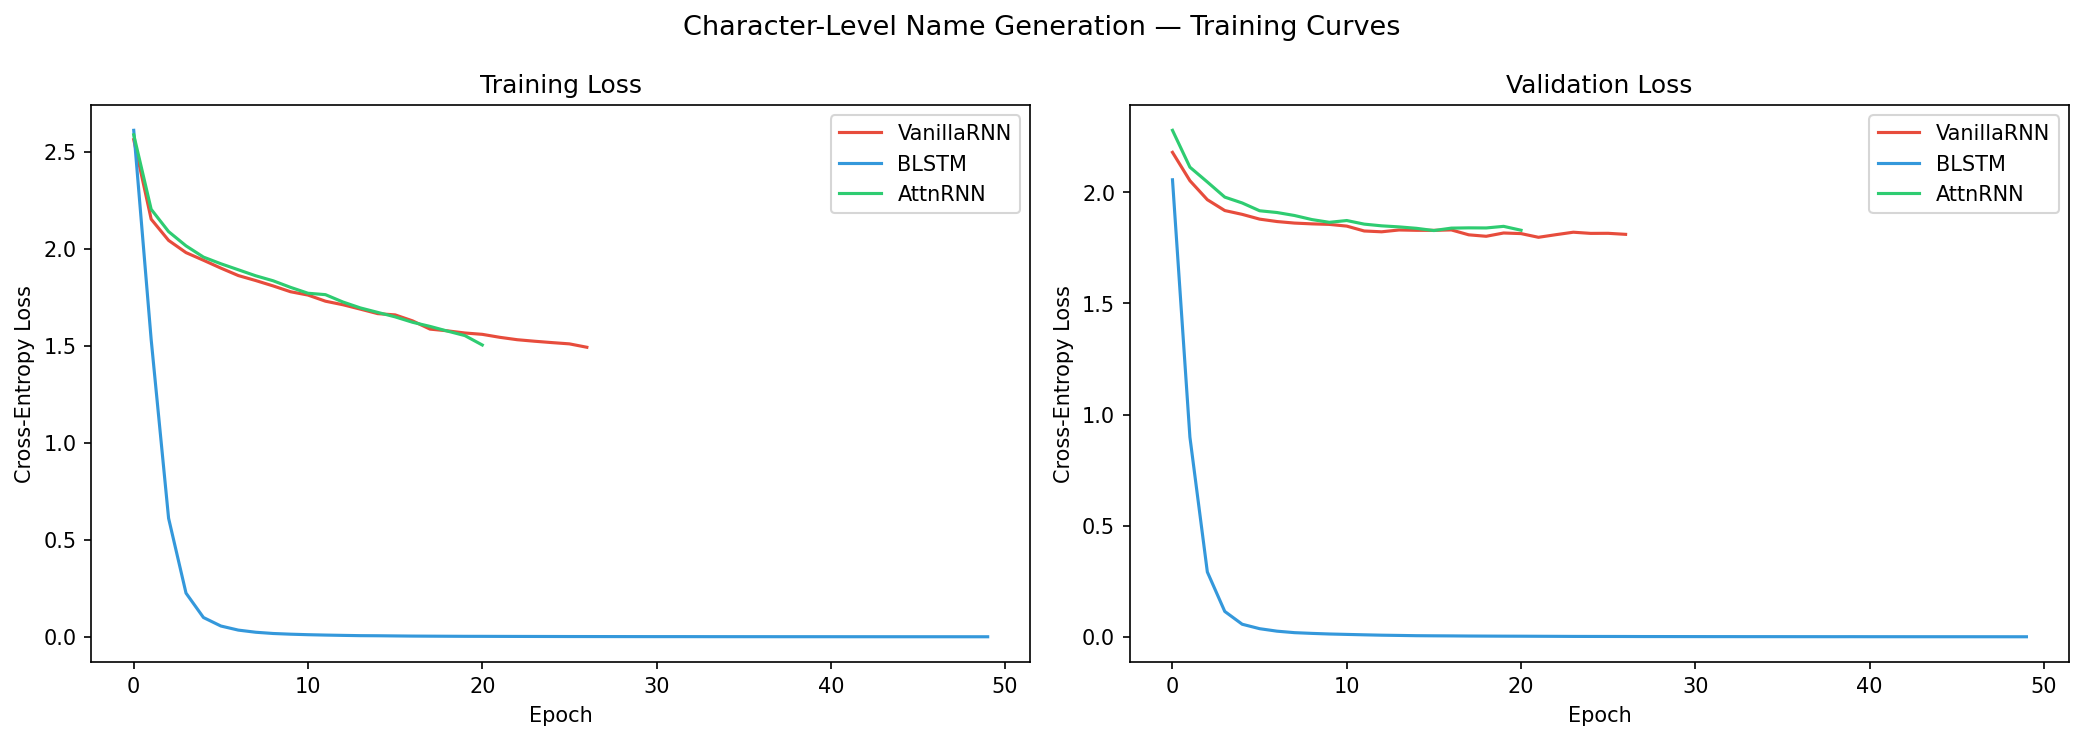
\includegraphics[width=\textwidth]{../plots/p2_training_loss.png}
    \caption{Training and validation loss curves for all three models. The BLSTM's validation loss collapses to near zero due to bidirectional training, while VanillaRNN and AttnRNN converge to comparable validation losses around 1.80.}
    \label{fig:training_loss}
\end{figure}

% ==============================================================
\section{Conclusion}
% ==============================================================

In this assignment we implemented Word2Vec from scratch and three character-level name generation models from scratch in PyTorch. Key takeaways:

\begin{enumerate}
    \item Word2Vec trained on a small 23k-token corpus produces noisy embeddings. Several target query words (\textit{exam}, \textit{btech}) were absent from the vocabulary entirely. The hyperparameter sweep reveals that $K=5$ negative samples works best on small corpora; more negative samples hurt performance by diluting the gradient signal.
    \item For character-level generation, VanillaRNN produces the most realistic Indian names, outperforming the more complex BLSTM on generation quality. This is a counterintuitive result explained by the bidirectional training/unidirectional generation mismatch in BLSTM.
    \item The attention mechanism (AttnRNN) produces names with reasonable phonetic structure but tends to generate longer outputs than VanillaRNN.
    \item Gradient clipping (at 5.0) is essential for training vanilla RNNs: without it, the loss diverges to NaN within a few batches.
    \item The forget gate bias initialisation to 1.0 in the custom LSTM cell is a small but impactful detail that significantly speeds up early training convergence.
\end{enumerate}

% ==============================================================
\bibliographystyle{plain}
\bibliography{refs}

\end{document}
